\draft Question on Josephson Junction and its application on B field measurement.

\begin{parts}
	\part $\phi$ is the phase difference of the 2 SC wavefunctions across the junction.
	
	The origin of the JJ equations:
	\begin{itemize}
		\item
		\begin{figure}[H]
			\centering
			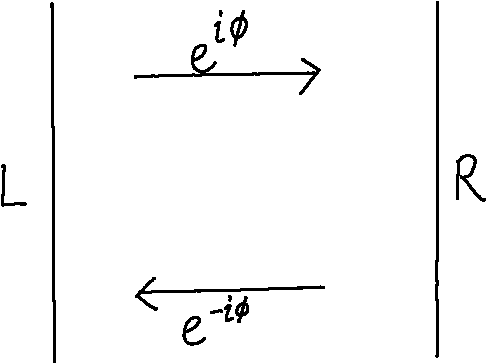
\includegraphics[width=.3\linewidth]{q6-tunnel}
		\end{figure}
		JJ1 -- consider the tunnelling from L$\rightarrow$R + R$\rightarrow$L:
		\begin{align*}
			I &\propto \mathrm{e}^{i\rbracket{\phi_2 - \phi_1}} - \mathrm{e}^{i\rbracket{\phi_1 - \phi_2}} \\
			&\propto \sin\phi \mtext{where\hspace{1em}} \phi = \phi_2 - \phi_1
		\end{align*}
		
		\item JJ2 -- consider TDSE on each side of the junction:
		\begin{align*}
			i\hbar \pdiff{t} \ket{\psi} &= E \ket{\psi} \mtext{where $\ket{\psi} = \sqrt{n_s}\mathrm{e}^{i\theta}$ is the SC wavefunction} \\
			-\hbar\pderi{\theta}{t} \ket{\psi} &= E \ket{\psi}
		\end{align*}
		Subtracting the energies across the junction then yields:
		\begin{align*}
			\Delta E &= -\hbar\pderi{\theta}{t} = -2eV \\
			V &= \frac{\hbar}{2e} \pderi{\theta}{t}
		\end{align*}
		where $V$ is the voltage developed due to the energy difference carried by the Cooper pair.
	\end{itemize}
	
	\part Sketch of the circuit:
	\begin{figure}[H]
		\centering
		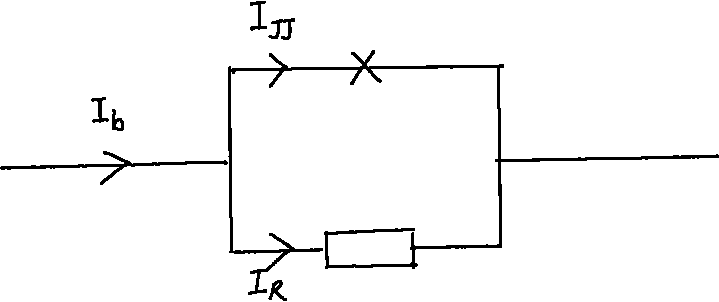
\includegraphics[width=.6\linewidth]{q6-circuit}
	\end{figure}
	
	KCL gives:
	\begin{align*}
		I_b &= I_{JJ} + I_R \\
		&= I_J \sin\phi + \frac{V}{R} \\
		&= I_J \sin\phi + \frac{\hbar}{2eR} \pderi{\phi}{t}
	\end{align*}
	
	For $I_b < I_J$, note we have a steady state solution: $\sin\phi = I_b/I_J$ so no voltage develops.
	
	For $I_b \ll I_J$, we have $\partial \phi/\partial t \simeq 2eR/\hbar I_b \Rightarrow V \simeq I_b R \Rightarrow$ Ohmic behaviour.
	
	Sketch of voltage against $I_b$:
	\begin{figure}[H]
		\centering
		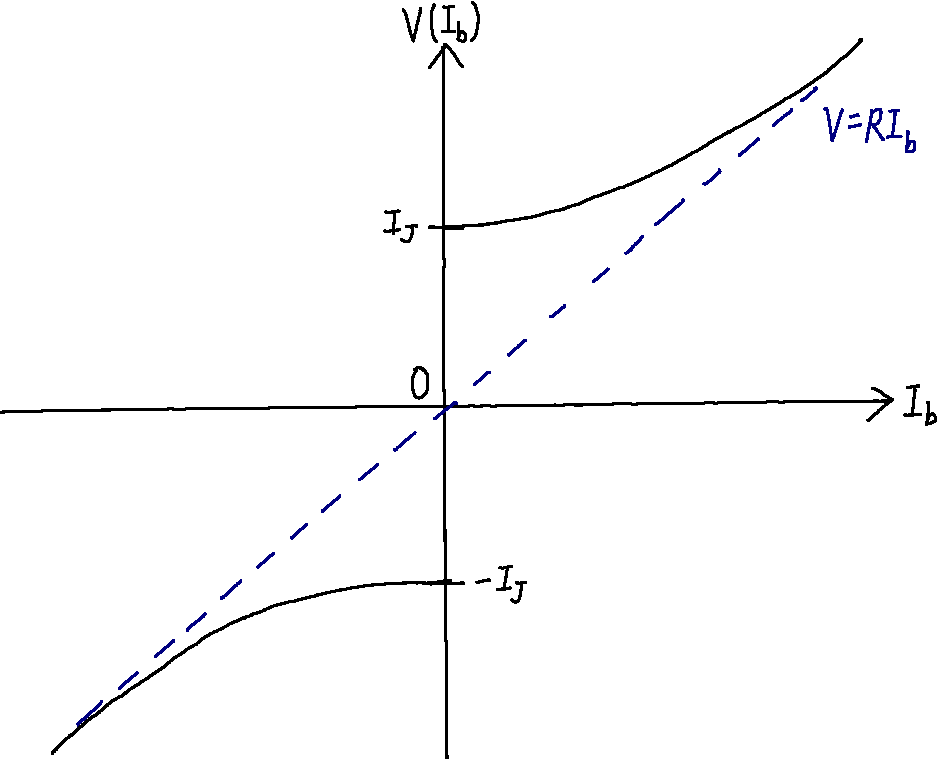
\includegraphics[width=.8\linewidth]{q6-vi}
	\end{figure}
	
	\part The flux dependence arises from the quantisation of flux through a loop of superconductors.
	This is due to the inherent rigidity of wavefunction where the phase must be single-valued upon a rotation of $2\pi$.
	
	2nd Ginzburg-Landau equation gives $\Phi_0$ as the flux quantum.
	
	\part \todo
	\begin{equation*}
		V = I_b R \sbracket{1 - \rbracket{\frac{I_J}{I_b}}^2}^{1/2}
	\end{equation*}
	So:
	\begin{align*}
		\pderi{V}{I_b} &= 0 = R \sbracket{1 - \rbracket{\frac{I_J}{I_b}}^2}^{1/2} + \frac{1}{2} I_b R \sbracket{1 - \rbracket{\frac{I_J}{I_b}}^2}^{-1/2} \rbracket{-2 \rbracket{\frac{I_J}{I_b}} \rbracket{-\frac{I_J}{I_b^2}}} \\
		&\Rightarrow R\sbracket{1 - \rbracket{\frac{I_J}{I_b}}^2} + I_b R \rbracket{\frac{I_J^2}{I_b^3}} = 0 \\
		???
	\end{align*}
	\begin{align*}
		\pderi{V}{\Phi} = I_b R \cdot \frac{1}{2} \sbracket{1 - \rbracket{\frac{I_J}{I_b}}^2}^{-1/2} \cdot \rbracket{-2 \frac{I_J}{I_b^2}} \rbracket{\pderi{I_J}{\Phi}}
	\end{align*}
	\begin{align*}
		\pderi{I_J}{\Phi} = I_{J0} \abs{\sin\rbracket{\frac{2\pi\Phi}{\Phi_0}}} \cdot \frac{2\pi}{\Phi_0}
	\end{align*}
	
	\part \todo So bias current???
\end{parts}